% \documentclass[UTF8,oneside]{ctexbook}
% \usepackage{pgfplots}
% \usepackage{caption}
% \begin{document}

\begin{figure}[!h]
% \centering

\makebox[\textwidth][c]{%
    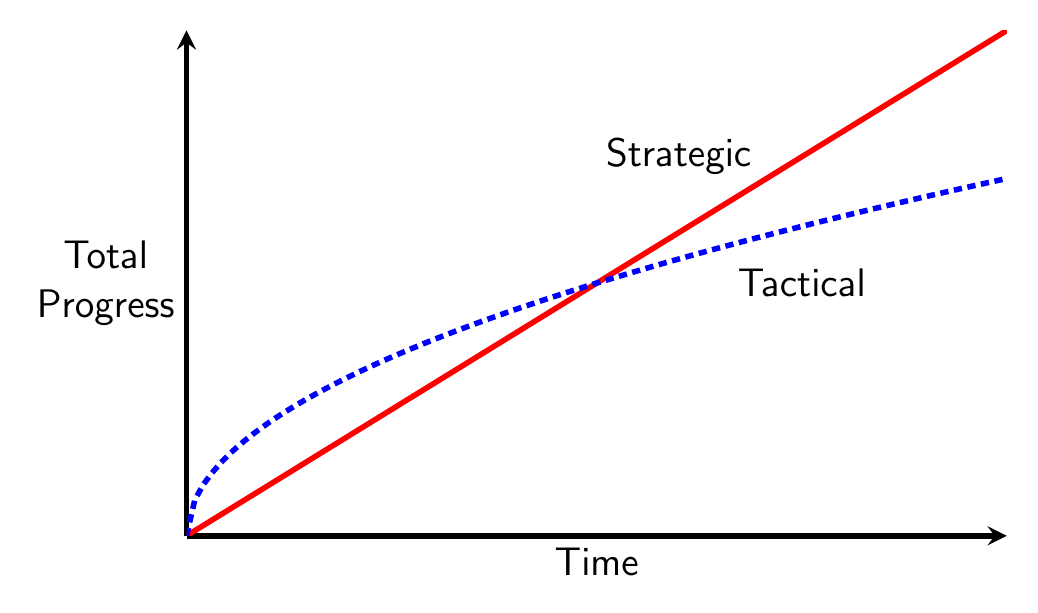
\begin{tikzpicture}[
        font = \sffamily\Large,
        every path/.append style ={line width = 2pt,},
    ]
    \begin{axis}[
        width = 12cm,
        height = 8cm,
        ticks = none,
        axis lines = left,
        xlabel = { Time } ,
        ylabel = { Total\\Progress },
        ylabel style = { rotate = -90, align  = center,},
    ]
    \addplot [domain=0:2,samples=100,color=red ] {x};
    \addplot [
        domain  = 0:2,
        samples = 100,
        color   = blue,
        densely dashed
    ] {x^0.5};
    \node[] at (axis cs: 1.2,1.5) { Strategic};
    \node[] at (axis cs: 1.5,1.0) { Tactical };
    \end{axis}
    \end{tikzpicture}
}%

\caption*{图 3.1}
\label{fig:3-1}
\end{figure}

% \end{document}